\chapter{Flight phases}
\label{ch:phases}
% Generated by scripts/reporting/ch4_flight_phases/generate_decoder_audit.py; match the audited snapshot.
\newcommand{\SegAuditParaCoherenceSD}{0.0000889}
\newcommand{\SegAuditParaExcludedPct}{8.24}
\newcommand{\SegAuditHangCoherenceSD}{0.0000604}
\newcommand{\SegAuditHangExcludedPct}{5.88}
\newcommand{\SegAuditReferenceClimb}{6}
\newcommand{\SegAuditPriorClimb}{6}
\newcommand{\SegAuditCurrentClimb}{32}
\newcommand{\SegAuditArchiveStatus}{The saved archive uses the current decoder. The four-dimensional path is reconstructed from the same fitted parameters as a comparison.}
\newcommand{\SegAuditSupportStatus}{The feature masks include the propagated reconstruction support of the vertical Savitzky--Golay derivatives.}
\newcommand{\SegAuditFitStatus}{The selected fits do not both satisfy a finite, non-negative last gain below tolerance (Table~\ref{tab:segmentationaudit}). The software stopping flags therefore cannot establish convergence of these fits; covariance and refitting sensitivity remain to be checked.}
\newcommand{\SegAuditAnnotationStatus}{No human reference intervals were supplied to this audit, so it reports no independent classification scores.}


The global observables of Chapter~\ref{ch:global} constrain the motion of a complete
flight, but because they mix directed travel, searching and altitude recovery, they do
not identify which behaviour contributes to a particular scaling law. Segmentation
provides the missing conditional description: given a phase, how does the glider move,
how long does that phase last, and what happens next?

The aim here is to assign these phases reproducibly and establish how the labels can
be checked, bearing in mind that kinematics provide indirect evidence of behaviour:
a coloured climb on a trajectory remains an inference. We first build the probabilistic model and define its measured features, then examine its numerical behaviour and the independent
annotations needed to assess its accuracy.

\section{What the three phases mean}
\label{sec:segmentation}
We retain the three-state description used by Vilpellet et al.~\cite{vilpellet2026},
with labels $\mathcal S=\{\mathrm T,\mathrm S,\mathrm C\}$:
\begin{description}[style=nextline]
  \item[Transition (T).] Sustained directed travel between lift regions, usually with
  limited turning and altitude loss.
  \item[Search (S).] Exploratory turns, reversals or recentering without a sustained
  established climb. Search can be brief or absent between a transition and a climb.
  \item[Climb (C).] Sustained exploitation of lift, usually combining positive mean
  vertical speed and circling.
\end{description}
These definitions concern observable flight geometry rather than a pilot's unrecorded
intention, and allow departures from a fixed cycle: a glider may encounter lift directly, leave
an unsuccessful search, or interrupt a climb. Ridge soaring and straight flight in rising
air may also be ambiguous within this three-state vocabulary. Such cases should remain
visible during validation instead of being forced to confirm the proposed interpretation.

\begin{figure}[tb]
\centering
\begin{tikzpicture}[schematic, x=1cm, y=1cm,
    panel/.style={rounded corners=2pt, line width=0.7pt}]
  % Three plan views, one per phase, in the phase colours of the plotted figures.
  \draw[panel, draw=phasetransition!55, fill=phasetransition!5] (0,0) rectangle (4.6,2.8);
  \draw[panel, draw=phasesearch!55, fill=phasesearch!6] (5.2,0) rectangle (9.8,2.8);
  \draw[panel, draw=phaseclimb!55, fill=phaseclimb!5] (10.4,0) rectangle (15.0,2.8);
  \node[panel title, text=phasetransition] at (0,3.15) {Transition};
  \node[panel title, text=phasesearch] at (5.2,3.15) {Search};
  \node[panel title, text=phaseclimb] at (10.4,3.15) {Climb};

  \draw[phasetransition, line width=1.2pt, ->]
    (0.45,1.15) .. controls (1.85,1.45) and (3.05,1.2) .. (4.15,1.75);
  \draw[phasesearch, line width=1.2pt, ->]
    (5.62,1.0) .. controls (8.16,0.9) and (8.89,2.05) .. (7.20,1.95)
             .. controls (5.87,1.8) and (6.71,1.1) .. (9.25,1.35);
  \draw[phaseclimb, line width=1.2pt, domain=0:780, samples=120, variable=\a, ->]
    plot ({12.6+0.78*cos(\a)+0.0005*\a},{1.5+0.56*sin(\a)});

  \node[fig note, anchor=south] at (2.3,0.25) {directed progress};
  \node[fig note, anchor=south] at (7.5,0.25) {exploratory turns};
  \node[fig note, anchor=south] at (12.7,0.25) {turning and ascent};

  \draw[->, black!45, line width=0.7pt] (4.65,1.4) -- (5.15,1.4);
  \draw[->, black!45, line width=0.7pt] (9.85,1.4) -- (10.35,1.4);
  \draw[->, black!45, line width=0.7pt, densely dashed]
    (2.3,-0.05) -- (2.3,-0.75) -- (12.7,-0.75) -- (12.7,-0.05);
  \node[fig note, fill=white, inner sep=3pt] at (7.5,-0.75) {search can be skipped};
\end{tikzpicture}
\caption{Schematic plan views of the three phase interpretations. The drawings are
illustrations, not measured trajectories or decision rules. Climbing circles can drift,
and searching can cover substantial ground; neither phase is assumed stationary.}
\label{fig:phasegeometry}
\end{figure}

\section{From a Markov chain to hidden-state inference}
\label{sec:hmmtheory}

The phase of a flight is not observed directly: a recorder measures motion, and different
behaviours can produce overlapping ranges of speed and turning. A hidden Markov model
represents this distinction through two coupled sequences. The latent sequence $Q_k$
describes the state at decision time $k$, while the observed vector $\mathbf Y_k$ carries
the measurements associated with that state. The construction and inference below follow
the standard HMM formulation~\cite[Secs.~II--III]{rabiner1989}; its use for behavioural
interpretation requires additional care, as discussed by McClintock et al.~\cite{mcclintock2020}.

\subsection{Constructing the probability law}

Begin with a chain on a finite state space $\mathcal S$. Its initial distribution and
transition probabilities satisfy
\begin{equation}
 \begin{aligned}
 \Pr(Q_1=i)&=\pi_i,&\sum_i\pi_i&=1,\\
 \Pr(Q_{k+1}=j\mid Q_{1:k-1},Q_k=i)&=a_{ij},&\sum_j a_{ij}&=1.
 \end{aligned}
 \label{eq:hmm-markov}
\end{equation}
Here $a_{ij}=\Pr(Q_{k+1}=j\mid Q_k=i)$ and all probabilities are nonnegative. The Markov assumption concerns the hidden state:
its present value contains the information about its history used to predict the next
state. A constant matrix $A$ adds time homogeneity; it is a modelling choice, not a
consequence of the observations being sampled regularly.

Now attach an emission density $b_i(\mathbf y)$ to each state, with
$\int b_i(\mathbf y)\,\mathrm d\mathbf y=1$. Conditional on the complete state sequence,
the emissions are assumed independent and the density at time $k$ depends only on $Q_k$.
The chain rule then gives
\begin{equation}
 p(q_{1:K},\mathbf y_{1:K}\mid\theta)
 =\pi_{q_1}b_{q_1}(\mathbf y_1)
   \prod_{k=1}^{K-1}a_{q_kq_{k+1}}b_{q_{k+1}}(\mathbf y_{k+1}),
 \label{eq:hmmjoint}
\end{equation}
where $\theta$ collects $\pi$, $A$ and the emission parameters. This is also a generative
recipe: draw the first state, generate its observation, then alternate a state transition
with a new observation. Although emissions are independent conditional on the states,
the observed sequence is generally correlated and need not itself be first-order Markov.

\begin{figure}[tb]
 \centering
 \begin{tikzpicture}[schematic, node distance=1.5cm,
     latent/.style={circle, draw=figblue, line width=0.8pt, fill=figblue!6,
                    minimum size=1.05cm},
     observed/.style={rectangle, rounded corners=1.5pt, draw=black!55, line width=0.8pt,
                      fill=black!5, minimum width=1.1cm, minimum height=0.85cm}]
  \node[latent] (q1) {$Q_{k-1}$};
  \node[latent,right=2cm of q1] (q2) {$Q_k$};
  \node[latent,right=2cm of q2] (q3) {$Q_{k+1}$};
  \node[observed,below=1.2cm of q1] (y1) {$\mathbf Y_{k-1}$};
  \node[observed,below=1.2cm of q2] (y2) {$\mathbf Y_k$};
  \node[observed,below=1.2cm of q3] (y3) {$\mathbf Y_{k+1}$};
  \draw[->, black!55, line width=0.7pt] (q1) -- node[above, fig tick, text=black!70] {$A$} (q2);
  \draw[->, black!55, line width=0.7pt] (q2) -- node[above, fig tick, text=black!70] {$A$} (q3);
  \draw[->, black!55, line width=0.7pt] (q1) -- node[right, fig tick, text=black!70] {$b_{Q_{k-1}}$} (y1);
  \draw[->, black!55, line width=0.7pt] (q2) -- node[right, fig tick, text=black!70] {$b_{Q_k}$} (y2);
  \draw[->, black!55, line width=0.7pt] (q3) -- node[right, fig tick, text=black!70] {$b_{Q_{k+1}}$} (y3);
  \node[left=.5cm of q1, align=right, fig note] {hidden\\states};
  \node[left=.5cm of y1, align=right, fig note] {observed\\features};
 \end{tikzpicture}
 \caption{Conditional structure of an HMM. Horizontal arrows carry state persistence
 and transitions; vertical arrows describe how a state generates a measurement. Absence
 of an arrow between observations represents conditional independence given the hidden
 sequence, not independence of the observed features over time.}
 \label{fig:hmm-graph}
\end{figure}

For continuous features, a common emission model is a multivariate Gaussian,
\begin{equation}
 b_i(\mathbf y)=\frac{\exp[-\tfrac12(\mathbf y-\boldsymbol\mu_i)^{\mathsf T}
                  \Sigma_i^{-1}(\mathbf y-\boldsymbol\mu_i)]}
 {(2\pi)^{d/2}|\Sigma_i|^{1/2}},\qquad \Sigma_i\succ0.
 \label{eq:hmm-gaussian-density}
\end{equation}
Its full covariance describes dependence among simultaneous features within a state.
Gaussianity is an additional assumption about the emission shape; it is not part of the
definition of an HMM. Nor does a state number determine a behavioural name: permuting
all state labels consistently leaves the observation law unchanged.

\subsection{Likelihood and uncertainty about the states}

Three tasks must be distinguished: evaluating how well given parameters explain an
observed sequence, inferring its hidden states, and estimating the parameters themselves.
For the first, the states must be summed out,
\begin{equation}
 \mathcal L(\theta)=p(\mathbf y_{1:K}\mid\theta)
 =\sum_{q_{1:K}\in\mathcal S^K}p(q_{1:K},\mathbf y_{1:K}\mid\theta).
 \label{eq:hmm-likelihood}
\end{equation}
With continuous observations this is a density evaluated at the recorded vectors, rather
than the probability of those exact vectors. Direct evaluation would enumerate
$|\mathcal S|^K$ paths, but the Markov factorization allows their shared prefixes and
suffixes to be accumulated recursively~\cite[Sec.~III-A]{rabiner1989}.

For one valid block of $K$ observations, define forward and backward quantities
\begin{align}
 \alpha_1(i)&=\pi_i b_i(\mathbf y_1),&
 \alpha_{k+1}(j)&=b_j(\mathbf y_{k+1})\sum_i\alpha_k(i)a_{ij},
 &\mathcal L&=\sum_i\alpha_K(i),\label{eq:forward}\\
 \beta_K(i)&=1,&
 \beta_k(i)&=\sum_j a_{ij}b_j(\mathbf y_{k+1})\beta_{k+1}(j).
 &&\label{eq:backward}
\end{align}
Their cost is $O(K|\mathcal S|^2)$, in contrast to enumerating $|\mathcal S|^K$ paths.
The posteriors used in Baum--Welch are
\begin{equation}
 \gamma_k(i)=\frac{\alpha_k(i)\beta_k(i)}{\mathcal L},\qquad
 \xi_k(i,j)=\frac{\alpha_k(i)a_{ij}b_j(\mathbf y_{k+1})\beta_{k+1}(j)}{\mathcal L}.
\end{equation}

Here $\alpha_k(i)$ is the joint density of the observations up to $k$ and state $i$,
whereas $\beta_k(i)$ is the conditional density of the remaining observations given that
state. Their product combines evidence on both sides of the decision. Thus
$\gamma_k(i)$ is a smoothed state probability, while $\xi_k(i,j)$ gives the expected
weight of a transition $i\to j$. Summing $\gamma_k$ over states, or $\xi_k$ over both
indices, gives one; no most-probable path needs to be selected to calculate them.

\subsection{Decoding a whole sequence}

Choosing $\arg\max_i\gamma_k(i)$ separately at every time maximizes the expected number
of correct individual states, but those choices need not form the most probable joint
sequence and can even violate a forbidden transition. Viterbi instead retains the best
path ending in each state~\cite{viterbi1967,rabiner1989}. In logarithmic form,
\begin{align}
 d_1(j)&=\log\pi_j+\log b_j(\mathbf y_1),\\
 d_{k+1}(j)&=\log b_j(\mathbf y_{k+1})+
                    \max_i[d_k(i)+\log a_{ij}],\\
 \psi_{k+1}(j)&=\arg\max_i[d_k(i)+\log a_{ij}].
 \label{eq:viterbi-recursion}
\end{align}
After choosing $\widehat q_K=\arg\max_jd_K(j)$, backtracking through
$\widehat q_k=\psi_{k+1}(\widehat q_{k+1})$ recovers the optimal sequence. Zero
probabilities have log score $-\infty$; ties require a consistent convention.
The forward recursion adds competing paths, while Viterbi takes their maximum, which
explains why a decoded path and posterior uncertainty are different outputs. Both
are conditional on the adopted model, so a high posterior does not independently
establish that a behavioural interpretation is correct.

\subsection{Learning from unlabelled observations}

If states were observed, transitions could be counted and each Gaussian fitted to its
assigned measurements. With hidden states, Baum--Welch replaces those unknown assignments
by their posterior weights and iterates the calculation~\cite{baum1970}. This is an
expectation--maximization procedure: at iteration $r$, compute
\begin{equation}
 \mathcal Q(\theta\mid\theta^{(r)})
 =\mathbb E_{Q\mid\mathbf y,\theta^{(r)}}
       [\log p(Q,\mathbf y\mid\theta)],
 \qquad
 \theta^{(r+1)}\in\arg\max_\theta\mathcal Q(\theta\mid\theta^{(r)}).
 \label{eq:hmm-em-objective}
\end{equation}
The E step uses forward--backward probabilities; the M step maximizes the resulting
expected complete-data log likelihood. Its monotonicity follows from the EM lower-bound
argument under an exact M step~\cite{dempster1977}, but does not imply a global optimum.
For $B$ observation blocks treated as independent in the likelihood and indexed by $b$, the unregularized Gaussian
M step gives the following updates, provided each denominator is positive:
\begin{align}
 \pi_i^{\mathrm{new}}&=\frac1B\sum_{b=1}^B\gamma_{b,1}(i),&
 a_{ij}^{\mathrm{new}}&=
 \frac{\sum_b\sum_{k=1}^{K_b-1}\xi_{b,k}(i,j)}
      {\sum_b\sum_{k=1}^{K_b-1}\gamma_{b,k}(i)},\label{eq:baumwelch}\\
 \boldsymbol\mu_i^{\mathrm{new}}&=
 \frac{\sum_{b,k}\gamma_{b,k}(i)\mathbf y_{b,k}}
      {\sum_{b,k}\gamma_{b,k}(i)},&
 \Sigma_i^{\mathrm{new}}&=
 \frac{\sum_{b,k}\gamma_{b,k}(i)
 (\mathbf y_{b,k}-\boldsymbol\mu_i^{\mathrm{new}})
 (\mathbf y_{b,k}-\boldsymbol\mu_i^{\mathrm{new}})^{\mathsf T}}
 {\sum_{b,k}\gamma_{b,k}(i)}.
 \label{eq:baumwelchcovariance}
\end{align}

Initial-state counts use only the first observation of each block, and transition counts
stop at its penultimate observation, so no transition is invented across a gap. These
formulas explain the statistical fit; numerical scaling, regularization, initialization
and stopping rules must also be specified for the actual estimator. The next sections
make those choices for flight observations, rather than treating the general HMM theory
as evidence that this particular three-state interpretation is correct.

\section{From the cleaned flight to observations}
\label{sec:phasefeatures}
The input is the final trajectory of Chapter~\ref{ch:dataset}, with local position
$(E,N,z)$ and the smoothed velocity and acceleration components. Each preprocessing
segment defines a separate observation sequence, within which feature windows and
hidden-state transitions cannot cross an acquisition gap or an excluded quality interval.

A common decision interval $\Delta=\SI{10}{\second}$ gives the transition matrix the
same physical meaning for every flight, restricting the analysis to native cadences no
slower than this interval. At each decision time $t_k$, we first compute each scalar
feature at native fixes and linearly interpolate those values. Denoting this interpolant
by $\mathcal I[f]$, we average it over a centred window of width $W=\SI{30}{\second}$:
\begin{equation}
 \overline f(t_k)=\frac{1}{W}\int_{t_k-W/2}^{t_k+W/2}\mathcal I[f](u)\,\mathrm du,
 \qquad
 \mathbf X_k=\bigl(\overline v_z,\overline v_h,
                  \overline{|\omega|},C_\omega\bigr)(t_k).
 \label{eq:phasefeatures}
\end{equation}
The window suppresses fix-scale fluctuations while preserving manoeuvres over tens of
seconds; its width is a chosen measurement scale rather than a measured universal
thermalling period.
Although boundaries lie on a 10-s grid, the overlapping 30-s windows prevent a claim of
independent 10-s temporal resolution.

The horizontal speed and signed turn rate are
\begin{equation}
 v_h=\sqrt{v_E^2+v_N^2},\qquad
 \omega=\frac{v_Ea_N-v_Na_E}{v_E^2+v_N^2}
 \quad (v_h\ge\SI{1}{\metre\per\second}).
 \label{eq:turnrate}
\end{equation}
Below the stated speed floor the implementation sets $\omega=0$, because numerical
heading is unreliable when the horizontal velocity nearly vanishes. The fourth feature
measures whether turning retains its sign:
\begin{equation}
 C_\omega(t_k)=
 \frac{\left|\int_{t_k-W/2}^{t_k+W/2}\mathcal I[\omega](u)\,\mathrm du\right|}
      {\int_{t_k-W/2}^{t_k+W/2}\mathcal I[|\omega|](u)\,\mathrm du},
 \qquad 0\le C_\omega\le1,
 \label{eq:turncoherence}
\end{equation}
The denominator is an accumulated angle in radians. The code sets $C_\omega=0$ if
it is at most machine epsilon ($2^{-52}$ in float64), and clips floating-point round-off
to $[0,1]$. Turning in one direction
throughout the window gives $C_\omega=1$ even when its rate varies: coherence is not a
measure of circularity or of lift by itself. At a reversal between two fixes,
$\mathcal I[|\omega|]$ differs from $|\mathcal I[\omega]|$: the former is the
quantity the code integrates. The pointwise inequality
$|\mathcal I[\omega]|\le\mathcal I[|\omega|]$ proves the stated bound on
$C_\omega$.

For example, equal-duration turns at $+6$ and $-6$ degrees per second cancel in the
numerator and give $C_\omega=0$, despite a large mean absolute turn rate. Keeping the
positive sign throughout gives $C_\omega=1$; spending three quarters of a window at
$+6$ and one quarter at $-6$ gives $C_\omega=1/2$ in the ideal piecewise-constant limit.
Thus two different questions are measured: how much the heading turns, and how much
opposite turns cancel. Figure~\ref{fig:coherence-schematic} makes this distinction explicit.

\begin{figure}[tb]
 \centering
 \begin{tikzpicture}[schematic]
  % Three idealised turn-rate windows. x: time in the window (s); y: omega (deg/s).
  \foreach \ox/\pt/\coh in {0/{(a) One direction}/{$C_\omega=1$},
                            4.9/{(b) Balanced reversal}/{$C_\omega=0$},
                            9.8/{(c) Unequal reversal}/{$C_\omega=1/2$}} {
    \begin{scope}[shift={(\ox,0)}, x=0.14cm, y=0.18125cm]
      \node[panel title] at (0,10.6) {\pt};
      \draw[fig grid] (0,0) -- (30,0);
      \draw[fig axis] (0,-8) rectangle (30,8);
      \foreach \x in {0,15,30} {
        \draw[fig axis] (\x,-8) -- (\x,-8.7);
        \node[fig tick, anchor=north, inner sep=3pt] at (\x,-8.7) {\x};
      }
      \node[fig label, anchor=north] at (15,-11.8) {Time in the window [s]};
      \node[fig note, anchor=north] at (15,-16.8) {\coh};
    \end{scope}
  }
  % y ticks on the left-hand panel, and the axis label once
  \begin{scope}[x=0.14cm, y=0.18125cm]
    \foreach \y/\lb in {-6/{$-6$}, 0/{$0$}, 6/{$+6$}} {
      \draw[fig axis] (0,\y) -- (-0.9,\y);
      \node[fig tick, anchor=east, inner sep=3pt] at (-0.9,\y) {\lb};
    }
    \node[fig label, rotate=90, anchor=south] at (-4.6,0) {$\omega$ [deg\,s$^{-1}$]};
    \draw[figblue, line width=1.3pt] (0,6) -- (30,6);
  \end{scope}
  \foreach \ox/\tswitch in {4.9/15, 9.8/22.5} {
    \begin{scope}[shift={(\ox,0)}, x=0.14cm, y=0.18125cm]
      \foreach \y in {-6,0,6} \draw[fig axis] (0,\y) -- (-0.9,\y);
      \draw[figblue, line width=1.3pt]
        (0,6) -- (\tswitch,6) -- (\tswitch,-6) -- (30,-6);
    \end{scope}
  }
 \end{tikzpicture}
 \caption{Turning amount and directional coherence measure different properties.
 All three idealized windows have $\overline{|\omega|}=6$ degrees per second, but their
 coherence differs because opposite turns cancel in the signed integral. The jumps
 illustrate limiting waveforms; the data calculation integrates piecewise-linear
 interpolants of native-fix values as specified in Eqs.~\eqref{eq:phasefeatures}
 and~\eqref{eq:turncoherence}. No phase label follows from coherence alone.}
 \label{fig:coherence-schematic}
\end{figure}

\begin{table}[tb]
 \centering\small
 \caption{Quantities shown in the phase time-series figures. Feature windows are
 centred and 30 s wide; the plotted quantities retain physical units, before standardization.}
 \label{tab:phase-figure-quantities}
 \begin{tabularx}{\linewidth}{@{}lXl@{}}
 \toprule
 Axis & Mathematical quantity & Unit / range\\
 \midrule
 Altitude & $z(t_k)$ from the cleaned trajectory & m\\
 Vertical speed & $\overline v_z(t_k)$, Eq.~\eqref{eq:phasefeatures} & m\,s$^{-1}$, signed\\
 Horizontal speed & $\overline{\sqrt{v_E^2+v_N^2}}(t_k)$ & m\,s$^{-1}$, $\ge0$\\
 Absolute turn rate & $(180/\pi)\overline{|\omega|}(t_k)$ & deg\,s$^{-1}$, $\ge0$\\
 Coherence & $C_\omega(t_k)$, Eq.~\eqref{eq:turncoherence} & dimensionless, $[0,1]$\\
 Posterior & $\gamma_k(i)$ for $i\in\{\mathrm T,\mathrm S,\mathrm C\}$ & $[0,1]$, sum $=1$\\
 Phase strip & $\widehat q_k$ from the joint Viterbi path & T, S, C or unavailable\\
 \bottomrule
 \end{tabularx}
\end{table}

A complete safe window is required. Windows touching reconstructed altitude, a derivative influenced by that reconstruction,
or an edge derivative from preprocessing are unclassified, as are unsupported feature
edges. Influence includes the entire Savitzky--Golay vertical fitting window, including
its off-centre boundary fits.
The support includes the native fixes bracketing interpolated window endpoints.
Consequently even an unsafe fix just outside the nominal integration interval can
invalidate it. Grey in the figures means unavailable support; there is no posterior
confidence threshold that turns uncertain classifications grey.

\section{A probabilistic segmentation, and its assumptions}
\label{sec:gaussianhmm}
\subsection{The fitted hidden Markov model}
\label{sec:hmminference}
A separate continuous Gaussian HMM is fitted for each discipline, since speed and turning
scale differ between paragliders and hang gliders. Write $Q_k\in\mathcal S$ for the
hidden phase and $\mathbf Y_k$ for the features standardized by training-set means and
standard deviations. More explicitly, for the $n$ observations actually selected for
fitting and feature $j$,
\begin{equation}
 \bar x_j=\frac1n\sum_{k=1}^n x_{kj},\qquad
 s_j^2=\frac1n\sum_{k=1}^n(x_{kj}-\bar x_j)^2,\qquad
 Y_{kj}=\frac{X_{kj}-\bar x_j}{s_j}.
 \label{eq:phase-standardization}
\end{equation}
A numerically constant feature is rejected; the population divisor $n$, rather than
$n-1$, matches the stored standardizer. The same $\bar x_j,s_j$ are used on held-out
observations. The model parameters are an initial distribution $\pi$, a transition
matrix $A$, and a full Gaussian covariance and mean for each component:
\begin{equation}
 a_{ij}=\Pr(Q_{k+1}=j\mid Q_k=i),\quad \sum_j a_{ij}=1,
 \qquad
 b_i(\mathbf y)=\mathcal N_d(\mathbf y;\boldsymbol\mu_i,\Sigma_i).
 \label{eq:hmmtransition}
\end{equation}
Full covariance allows simultaneous vertical speed, horizontal speed and turning to be
correlated within a phase. It does not model residual correlation \emph{between}
successive observations. The factorization in Eq.~\eqref{eq:hmmjoint} assumes first-order phase memory,
time-homogeneous parameters and conditionally independent emissions.
The last is only approximate for overlapping windows; posterior confidence may therefore
be sharper than independent observations would justify. Gaussian emissions also place
some probability on physically impossible feature values, such as negative speed.
They are a classification approximation, not a generative model of flight physics.

Baum--Welch applies expectation--maximization to the unlabelled training
likelihood~\cite{baum1970,dempster1977}. Ten fixed-seed initializations
are compared by training likelihood. Whole valid blocks enter the fit; the final
observation of one block never contributes a transition to the next. The fitted scaler
is frozen for validation and test flights.

A numerical component has no behavioural name. At present the component with greatest
mean vertical speed is provisionally called climb. Among the other two components,
transition maximizes $\mu_{v_h}-\mu_{|\omega|}-\tfrac12\mu_{C_\omega}$
in standardized feature coordinates; the remaining component is called search. Human train labels will resolve this
permutation. In particular, ``search'' currently also collects observations unexplained
by the other two components: its behavioural interpretation requires a direct check.

\subsection{Numerical estimation in the fitted model}
\label{sec:hmmestimation}

Equations~\eqref{eq:baumwelch}--\eqref{eq:baumwelchcovariance} describe unregularized
maximum likelihood. The stored models were fitted with \texttt{hmmlearn} 0.3.3~\cite{hmmlearn033}. Its default initial/transition
Dirichlet parameters are one, and its mean weight is zero, so those updates reduce to
the expressions above. For full covariance the default scalar \texttt{covars\_prior}
is $0.01$, broadcast to every matrix entry. With $N_i=\sum_{b,k}\gamma_{b,k}(i)$,
the implemented covariance update is therefore
\begin{equation}
 \Sigma_i^{\rm new}
 =\frac{\sum_{b,k}\gamma_{b,k}(i)
    (\mathbf y_{b,k}-\boldsymbol\mu_i^{\rm new})
    (\mathbf y_{b,k}-\boldsymbol\mu_i^{\rm new})^{\mathsf T}
    +0.01\,\mathbf 1\mathbf 1^{\mathsf T}}{N_i}.
 \label{eq:hmmactualcovariance}
\end{equation}
The added matrix is rank one: it does not impose a positive lower bound on every
covariance eigenvalue. In particular, \texttt{min\_covar}$=10^{-3}$ is added to the
initial covariance diagonal; it is not enforced as an eigenvalue floor after every
M step. This distinction matters for the very narrow coherence component.

Exact unregularized EM cannot decrease its likelihood, but convergence of the
parameters to a stationary point requires further regularity conditions; a mixture
can approach a singular covariance. The software's stopping flag is also true when
the iteration cap is reached or the last likelihood change is negative. That flag in
an old artifact is not evidence of convergence. New fits record convergence only for
a finite, non-negative last gain below the tolerance, reject non-finite final scores,
and still retain all restart scores for inspection. For restart $r$, write $\ell_r=\sum_b\log\mathcal L_b(\widehat\theta_r)$ on the same
training observations. Its reported relative score is
$(\ell_r-\max_u\ell_u)/n\le0$, in natural-log units per fitted observation, whereas the
final EM gain is $\ell^{(m)}-\ell^{(m-1)}$ before normalization. These are numerical
fit diagnostics, not accuracy scores. Ten fixed-seed restarts are ranked
by finite training likelihood; a restart can be selected without satisfying the stated
convergence criterion. Training uses scaled forward--backward arithmetic; current
Viterbi and posterior decoding use logarithms to avoid underflow.


\subsection{Why the current decoder differs from the original fit}
\label{sec:phaseprovisional}
The original fit used all four features. Its climb component concentrates coherence
extremely close to one: the physical standard deviations are approximately
$\SegAuditParaCoherenceSD$ for paragliders and $\SegAuditHangCoherenceSD$ for hang gliders
(Table~\ref{tab:segmentationaudit}). A circling climb with a small turn reversal can
therefore receive negligible climb likelihood. More persistent transitions alone cannot
repair this emission problem.

The current decoder integrates coherence out of the original four-dimensional Gaussian.
If $\mathbf U=(Y_1,Y_2,Y_3)$ and $V=Y_4$, then
\begin{equation}
 b_i^{(3)}(\mathbf u)
 =\int_{\mathbb R} b_i^{(4)}(\mathbf u,v)\,\mathrm dv
 =\mathcal N_3(\mathbf u;\boldsymbol\mu_{i,U},\Sigma_{i,UU}).
 \label{eq:phasemarginal}
\end{equation}
Thus the retained mean entries and principal covariance submatrix define the new
likelihood. This is marginalization, not conditioning on perfect coherence, and not a
new three-dimensional fit. Coherence remains recorded and plotted for inspection.
A separately refitted three-dimensional model remains a validation comparison: the
original parameters were selected using the problematic fourth feature.

The coherence mean and width in Table~\ref{tab:segmentationaudit} undo the training
standardization: $\mu_{C,i}^{\rm phys}=\bar x_4+s_4\mu_{i,4}$ and
$\sigma_{C,i}^{\rm phys}=s_4\sqrt{\Sigma_{i,44}}$. They describe a fitted Gaussian
component, not the sample mean and standard deviation of decisions labelled climb.

A second, independent choice softens the phase sequence. With $s_i=a_{ii}<1$ and
$q_{ij}=a_{ij}/(1-s_i)$ for $j\ne i$, the decoding matrix is
\begin{equation}
 \widetilde a_{ii}=\widetilde s_i,\qquad
 \widetilde a_{ij}=(1-\widetilde s_i)
       \bigl[(1-w)q_{ij}+wq^\star_{ij}\bigr],\quad j\ne i.
 \label{eq:phaseprior}
\end{equation}
Here $w=0.75$. The target exits from transition split equally between search and climb,
allowing direct entry into lift; from search and climb, the next phase in
$\mathrm T\to\mathrm S\to\mathrm C\to\mathrm T$ receives target probability $0.95$.
The persistence rule is
\begin{equation}
 \widetilde s_i=
 \begin{cases}
 s_i+w\bigl(e^{-\Delta/\theta_S}-s_i\bigr),&i=\mathrm S,\\
 s_i+w\max\bigl(0,e^{-\Delta/\theta}-s_i\bigr),&i=\mathrm T,\mathrm C,
 \end{cases}
 \quad \theta_S=\SI{20}{\second},\quad\theta=\SI{120}{\second}.
 \label{eq:phasepersistence}
\end{equation}
For an absorbing fitted row ($s_i=1$), the code starts from equal exit weights and
caps the new persistence at $1-\epsilon_{\rm mach}$ to retain possible exits.
These scales and weights are provisional decoder settings. They are neither fitted
behavioural durations nor minimum run lengths. Figure~\ref{fig:phasedecodingmatrix}
shows both matrices so that learned structure and imposed preference can be distinguished.
Once a semantic prior is active, changing component names requires decoding again,
rather than merely recolouring an existing path.

\begin{figure}[tb]
 \centering
 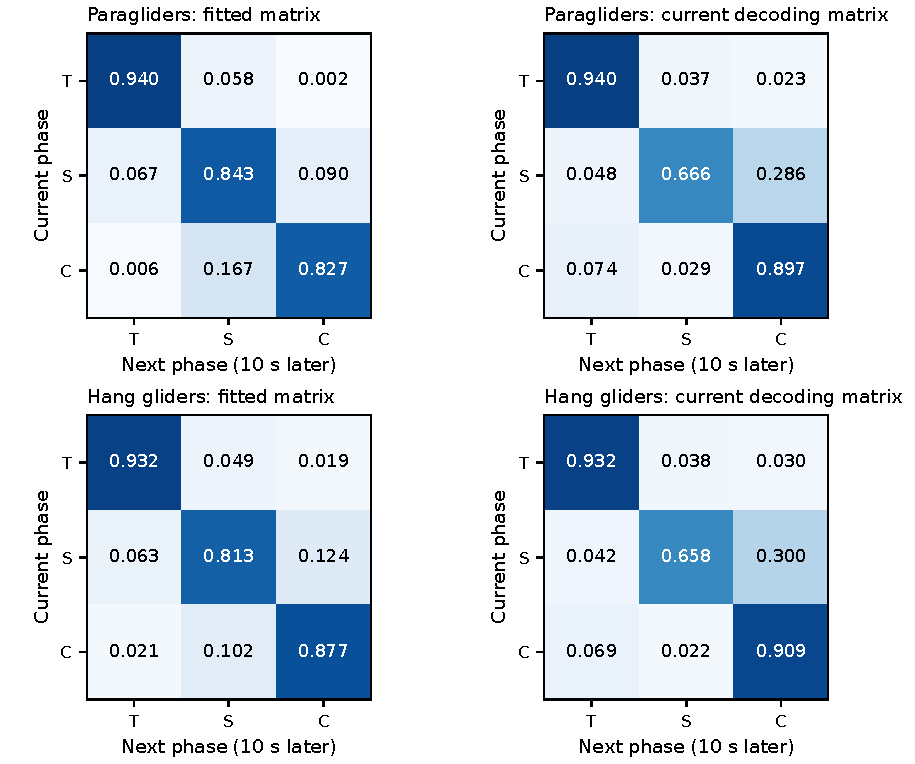
\includegraphics[width=\linewidth]{generated/segmentation_decoding_transitions.pdf}
 \caption{Original fitted and current decoding transition matrices, ordered as transition
 (T), search (S), climb (C). Every entry is a probability per 10-s decision. The right
 column includes the declared sequence preference and cannot be read as an empirical
 frequency of pilot behaviour.}
 \label{fig:phasedecodingmatrix}
\end{figure}

For both the original and modified model, Viterbi chooses the entire most probable
path rather than the most likely phase at each isolated time~\cite{viterbi1967}:
\begin{equation}
 \widehat q_{1:K}=\arg\max_{q_{1:K}}p(q_{1:K}\mid\mathbf y_{1:K}),\qquad
 \gamma_k(i)=\Pr(Q_k=i\mid\mathbf y_{1:K}).
 \label{eq:viterbi}
\end{equation}
The hard path and posterior $\gamma$ use the same effective transition matrix and
marginal emission. ``Smoothed posterior'' refers to inference using observations before
and after $k$, not to an extra filter applied to probabilities.

\section{What has been checked}
\label{sec:phasevalidation}
\subsection{Archive support and reproducible examples}
The original models were fitted and applied to both archives.
Table~\ref{tab:segmentationfit} records the actual fitting and decoding counts. Fitting
uses a deterministic subset of whole training blocks up to the memory cap; longer selected
blocks contribute more observations, so this is not equal weighting of flights.
\SegAuditArchiveStatus
The figures in this chapter use the current configuration and saved features,
with complete valid blocks decoded before an eight-minute display excerpt is taken.
A shortened figure therefore does not shorten the sequence used for inference.

% Generated by scripts/reporting/ch4_flight_phases/generate_segmentation_report.py -- do not edit.
\begin{table}[tb]
\centering
\small
\caption{Archive-scale HMM fit and decoding census.  A sequence is a contiguous classifiable feature block; restart numbers are one-based.}
\label{tab:segmentationfit}
\begin{tabular}{lrrrrr}
\toprule
Discipline & Fit flights & Fit sequences & Fit points & Decoded points & Restart \\
\midrule
Paragliders & \StatSegParaFitFlights & \StatSegParaFitSequences & \StatSegParaFitObservations & \StatSegParaDecodedPoints & \StatSegParaSelectedRestart/10 \\
Hang gliders & \StatSegHangFitFlights & \StatSegHangFitSequences & \StatSegHangFitObservations & \StatSegHangDecodedPoints & \StatSegHangSelectedRestart/10 \\
\bottomrule
\end{tabular}
\end{table}

% Generated by scripts/reporting/ch4_flight_phases/generate_decoder_audit.py; no accuracy implied.
\begin{table}[tb]
\centering\small
\caption{Support and numerical diagnostics of the segmentation. Excluded time uses all retained cleaned-segment duration as its denominator. Coherence widths belong to the original four-dimensional climb component.}
\label{tab:segmentationaudit}
\begin{tabular}{lrr}
\toprule
Quantity & Paragliders & Hang gliders \\
\midrule
Emitted archive decisions & 171{,}721{,}035 & 7{,}305{,}190 \\
Excluded cleaned duration & 8.28\% & 5.93\% \\
Climb $C_\omega$ mean (original fit) & 0.9999986 & 0.9999996 \\
Climb $C_\omega$ standard deviation & 0.0000889 & 0.0000604 \\
Final EM log-likelihood change & -0.223 & -0.253 \\
Annotated intervals supplied & 0 & 0 \\
\bottomrule
\end{tabular}
\end{table}


\SegAuditFitStatus

Coverage has a separate denominator from classification accuracy:
\begin{equation}
 f_{\mathrm{unclassified}}
 =1-\frac{\text{duration covered by classified decision cells}}
              {\text{total retained cleaned-segment duration}}.
 \label{eq:phasecoverage}
\end{equation}
Decision cells $[t_k-\Delta/2,t_k+\Delta/2)$ are clipped at segment boundaries;
acquisition gaps contribute to neither duration. For exclusion reason $r$, the plotted
percentage is $100\sum_k |I_k|\mathbf1\{r_k=r\}/D_{\rm clean}$, with $I_k$ the clipped
decision cell and $D_{\rm clean}$ the denominator in Eq.~\eqref{eq:phasecoverage}.
Feature-edge status takes precedence over a quality mask if both apply. Segments with
native cadence above 10 s contribute their full duration to the cadence category;
remaining tails outside any cell form the final category. The categories are disjoint. The denominator does include retained
segments too sparsely sampled for classification. The excluded fractions are \SegAuditParaExcludedPct\%
for paragliders and \SegAuditHangExcludedPct\% for hang gliders, chiefly from unsafe feature support
(Fig.~\ref{fig:phasecoverage}). These masks are shared by the two decoders compared on that snapshot.
\SegAuditSupportStatus Their coverage says how much time is available for subsequent phase statistics,
not whether any phase label is correct or whether exclusion is behaviourally unbiased.

\begin{figure}[tb]
 \centering
 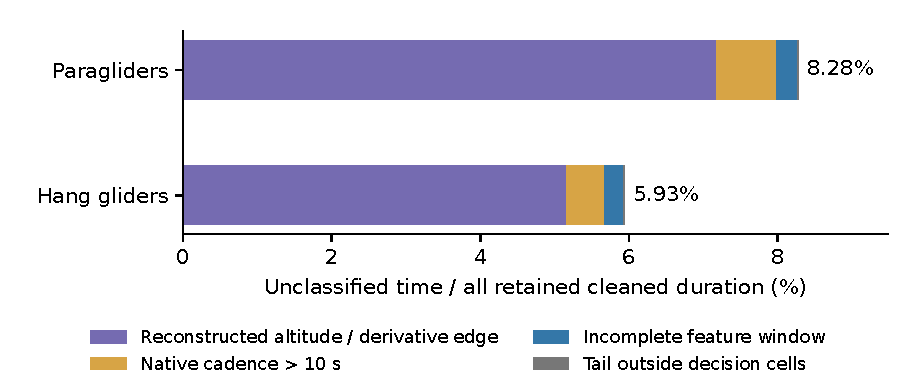
\includegraphics[width=\linewidth]{generated/segmentation_coverage.pdf}
 \caption{Why retained cleaned time lacks a phase label. Fractions use the same duration
 denominator in Eq.~\eqref{eq:phasecoverage}; they are not fractions of flights or fixes.
 Windows touching reconstructed altitude or edge derivatives dominate the excluded time.}
 \label{fig:phasecoverage}
\end{figure}

The two examples are selected by a fixed priority from validation flights, independently
of their apparent phase composition. Recomputing labels with the stored model reproduces the archived paths. Their current labels and posterior curves
then use Eqs.~\eqref{eq:phasemarginal}--\eqref{eq:phasepersistence}.
The audit records the selected identities, model hashes, configuration, and changed-label
counts. Thus each plotted label can be traced to its observations and decoder settings.

\begin{figure}[p]
 \centering
 
\includegraphics[width=\linewidth]{generated/segmentation_current_example_para.pdf}
 \caption{Eight minutes of a validation paraglider segment, decoded using the current
 three-feature marginal and sequence policy. The phase strip, altitude, separate feature
 axes and posterior probabilities share a time axis marked at one-minute intervals;
 decisions remain \SI{10}{\second} apart. Table~\ref{tab:phase-figure-quantities}
 defines every displayed quantity. Coherence is shown as a
 diagnostic and does not enter the current emission likelihood. Grey indicates unavailable
 support. Phase names remain provisional.}
 \label{fig:segmentationexamplepara}
\end{figure}
\begin{figure}[p]
 \centering
 
\includegraphics[width=\linewidth]{generated/segmentation_current_example_hang.pdf}
 \caption{The corresponding eight-minute hang-glider validation excerpt. It uses its own
 fitted model and standardizer, with the same feature definitions and display convention
 as Fig.~\ref{fig:segmentationexamplepara}. A high posterior expresses certainty within
 the adopted model; it is not an independently measured probability of correct behaviour.}
 \label{fig:segmentationexamplehang}
\end{figure}

The paraglider excerpt shows sustained turning and altitude recovery after an initial
transition, with a climb label that persists through brief changes in vertical speed
and coherence. The hang-glider excerpt is less clear-cut: part of a sustained ascent
is assigned to search, and the posterior divides between search and climb. Positive
vertical speed is therefore not equivalent to the fitted climb state. This could reflect
a difference in turning behaviour, but the figure alone cannot resolve the behavioural
name of that component. It gives a concrete interval for human validation rather than
an example selected to display apparently perfect classification.

The development example in Fig.~\ref{fig:phaseablation} separates the two decoder changes.
On its full preprocessing segment, the four-dimensional reference assigns \SegAuditReferenceClimb\ decisions to climb,
the sequence-only variant assigns \SegAuditPriorClimb, and the current
three-dimensional marginal assigns \SegAuditCurrentClimb. The comparison shows how the coherence coordinate and sequence preference affect
the same observations. The example helped motivate the change,
so the comparison is a regression diagnostic, not independent evidence of improved
accuracy. Neither a longer green interval nor a smaller number of switches is, by itself,
a success criterion.

\begin{figure}[tb]
 \centering
 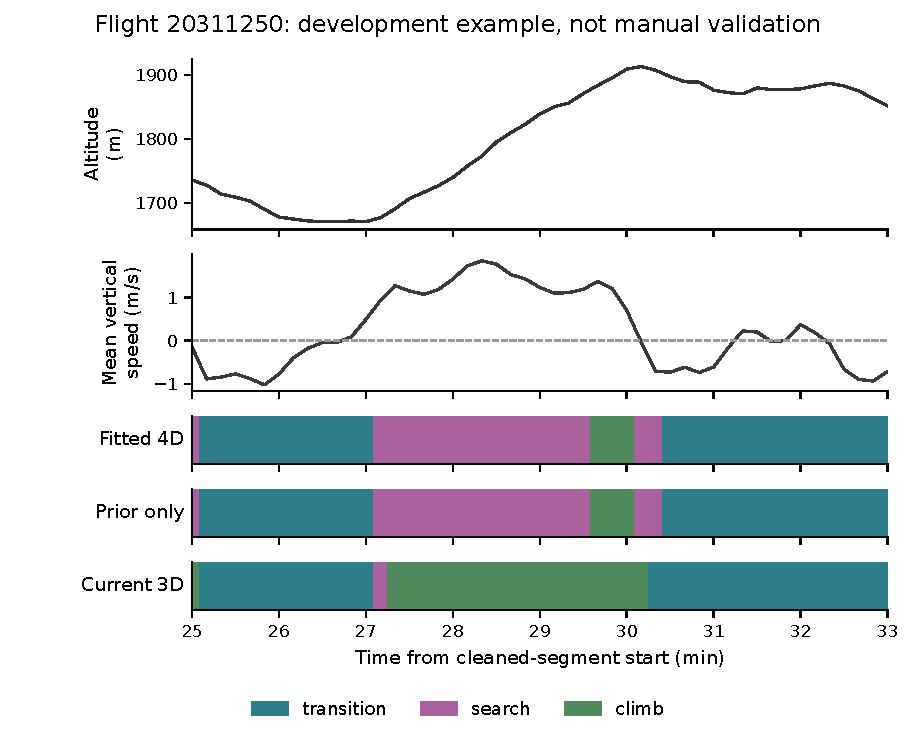
\includegraphics[width=\linewidth]{generated/segmentation_decoder_ablation.pdf}
 \caption{An eight-minute development excerpt from flight 20311250. The aligned phase
 strips compare the fitted four-dimensional reference, a change of sequence policy alone,
 and the current three-dimensional marginal with that policy. The altitude and vertical
 speed provide physical context. No human reference labels are present.}
 \label{fig:phaseablation}
\end{figure}

\subsection{The manual check that is still needed}
The prepared blinded pack contains 40 candidate flights: per discipline, four training
candidates, eight validation candidates and eight test candidates. Human reference intervals are needed before reporting accuracy, confusion matrices
or a definitive physical meaning for the search state. \SegAuditAnnotationStatus
The interactive tool is available: select an altitude interval and mark transition, search
or climb; edits are saved automatically on the 10-s decision grid. The plan view and
kinematics are visible, while model predictions are hidden. The pack must match the cleaned
archive used for evaluation; the regeneration procedure creates a new dated pack
while preserving the previous pack and any labels already written.

Clearly interpretable intervals should be labelled across the whole candidate window;
ambiguous boundaries can remain unlabelled. The fraction left unlabelled must accompany
the scores, since evaluating only easy interiors would otherwise conceal the difficult
part of segmentation. A second independent annotation of a subset will measure human
agreement and boundary ambiguity. That agreement study has not yet been performed.

The deterministic 70/15/15\% split operates at flight level, so no flight is shared
between fitting and nominal holdout sets. This alone does not guarantee an untouched
test: development flights 20275040 and 20279877 were inspected despite belonging to
the nominal test partition. They, and hang-glider example flight 975, are excluded from the prepared annotation
test pack and must remain outside final accuracy claims. Repeated pilots, days or sites can also
make flights statistically related; generalization to a new region or season requires
an additional grouped holdout, rather than being inferred from a random flight split.

Train annotations resolve state naming; validation annotations compare the original
four-dimensional model, the marginal decoder with and without the sequence preference,
and a refitted three-dimensional model. Model choices are then frozen before test
scores are opened. For human label $i$ and inferred label $j$, let $n_{ij}$ count
classified, annotated decisions. The core metrics are
\begin{equation}
 \begin{aligned}
 \mathrm{Precision}_i&=\frac{n_{ii}}{\sum_jn_{ji}},&
 \mathrm{Recall}_i&=\frac{n_{ii}}{\sum_jn_{ij}},\\
 F_{1,i}&=\frac{2n_{ii}}{\sum_jn_{ji}+\sum_jn_{ij}},&
 F_{1,\mathrm{macro}}&=\frac13\sum_iF_{1,i}.
 \end{aligned}
 \label{eq:phasevalidationmetrics}
\end{equation}
If a precision, recall or F1 denominator is zero, the evaluator assigns that metric
zero and retains the phase in the three-state macro average.
The corresponding accuracy is
$\mathrm{Acc}=\sum_i n_{ii}/\sum_{ij}n_{ij}$ on the same annotated, classified decisions;
the evaluator requires at least one annotated, classified decision. On that
nonempty set all these classification scores lie in $[0,1]$. The confusion matrix reveals whether search is systematically confused with climbing or
transition; macro-F1 gives a rare phase the same weight as a frequent one. Accuracy alone
can be dominated by the most occupied phase. Bootstrap intervals~\cite{efron1979}
obtained by resampling whole flights preserve
within-flight dependence, although they do not remove dependence between related flights.
The existing evaluator provides these classification metrics. Boundary errors, annotation
coverage and between-observer agreement remain additional validation measurements to
complete; no values are supplied before labels exist.

\section{What the segmentation will let us measure}
\label{sec:phaseobs}
The next empirical chapter will characterize all three phases before selecting a
stochastic transport model. For a phase occurrence $I=[a,b)$, useful primitive quantities
are its duration $D=b-a$, horizontal path length $L$, net displacement $R$, and altitude
change:
\begin{equation}
 L=\int_a^b v_h(t)\,\mathrm dt,\qquad
 R=\|\mathbf r(b)-\mathbf r(a)\|,\qquad
 \Delta z=z(b)-z(a),\qquad
 \mathcal P=R/L\in[0,1]\quad(L>0).
 \label{eq:phaseprimitives}
\end{equation}
Here $\mathbf r=(E,N)$ and $v_h=\|\dot{\mathbf r}\|$ refer to the same
horizontal curve; this consistency is needed for the triangle inequality $R\le L$.
The discrete implementation must use a matching position-based path length rather
than assume that separately smoothed derivatives satisfy the inequality exactly.
The ratio $\mathcal P$ distinguishes local circling from directed progress without
assuming that either occurs in a particular phase. The ground displacement of a climb
can be substantial in wind; search is not automatically an immobile waiting state.
Distributions of $(D,L,R,\Delta z)$ and phase-conditioned velocity correlation will
quantify those differences.

A phase-conditioned MSD requires an explicit conditioning convention. One useful choice
keeps the \emph{entire} displacement interval inside a single occurrence of phase $i$:
\begin{equation}
 M_i(\tau)=
 \frac{\sum_I\int_{a_I}^{b_I-\tau}
       \|\mathbf r(t+\tau)-\mathbf r(t)\|^2\,\mathrm dt}
      {\sum_I(D_I-\tau)_+},
 \qquad I\text{ an occurrence of phase }i.
 \label{eq:phaseconditionalmsd}
\end{equation}
Integrals for $D_I\le\tau$ contribute zero, and the observable is defined only
when its denominator is positive. This weights eligible time origins;
long occurrences contribute more, and short occurrences disappear at large lags.
A plot must therefore show the contributing occurrences and durations, and be checked
against equal-occurrence or equal-flight weighting. Conditioning only the two endpoints
would define a different observable because it could cross other phases.

\label{sec:reproducing}
Prior phase-resolved results~\cite{vilpellet2026} supply comparisons, not values that the
segmenter must be tuned to recover. Agreement in phase MSDs or time budgets cannot
independently validate a classifier designed around the same kinematic expectations.
Differences in sampling, geography, wind and the phase definitions must be considered
before attributing a disagreement to the dynamics.

\subsection{Keeping model assumptions separate from measured physics}
\label{sec:modelling}
An HMM imposes a geometric latent dwell-time law. With decoding persistence
$\widetilde a_{ii}$, its model prediction is
\begin{equation}
 \Pr(D_i=m\Delta)=\widetilde a_{ii}^{\,m-1}(1-\widetilde a_{ii}),\qquad
 \mathbb E[D_i]=\frac{\Delta}{1-\widetilde a_{ii}}.
 \label{eq:hmmsojourn}
\end{equation}
for $m=1,2,\ldots$ and $0\le\widetilde a_{ii}<1$.
A Viterbi run-length histogram is not a sample of observed physical durations independent
of this assumption. It depends on the emissions and the decoder as well as on behaviour.
Runs cut by a gap, quality mask or feature boundary are censored; merely discarding them
can bias the surviving duration distribution. Testing non-geometric phase durations
requires human reference intervals and a sensitivity analysis against a model with
explicit duration distributions, such as a hidden semi-Markov model~\cite{langrock2012}.
The imposed exit preferences likewise prevent interpreting the current decoded phase
order as unqualified evidence of physical memory.

The later transport model must reproduce both these phase observables and the global
constraints of Chapter~\ref{ch:global}. In particular, the duration of a moving leg and
its displacement should be studied jointly. A constant-speed L\'evy walk couples a leg's
length to that \emph{same leg's travel time}; dependence between its length and a
\emph{subsequent} climb or search is a separate question. A stereotyped phase cycle by
itself also does not disprove renewal at the level of complete cycles. Renewal requires
independence of successive cycle variables, which must be tested at the chosen event
scale.

\section{Chapter summary}
\label{sec:tooling}
The chapter has built the hidden-state model from its probability law, connected each
feature to a measured kinematic quantity, and separated parameter fitting from sequence
decoding. The current labels use a three-feature marginal of a fitted four-feature
Gaussian HMM and an explicit sequence preference. Coverage, numerical diagnostics,
short trajectory excerpts and a decoder comparison make those choices inspectable,
without supplying an independent estimate of behavioural accuracy. The current archive
leaves \SegAuditParaExcludedPct\% of retained paraglider time and
\SegAuditHangExcludedPct\% of hang-glider time unclassified. The narrow coherence
components and negative final likelihood changes remain numerical limitations, while
the ascent labelled search in the hang-glider example exposes a behavioural ambiguity
that posterior probabilities cannot settle.

The next step is the independent phase validation. Once its errors and boundary
uncertainties are known, phase durations, displacements and correlations can be used
alongside the global observables to test a physical transport model.
